\documentclass[11pt]{article}
\usepackage[a4paper, text={17cm, 24cm}, left=2cm, top=3cm]{geometry}
\usepackage[utf8]{inputenc}
\usepackage[T1]{fontenc}
\usepackage[slovak]{babel}
\usepackage{csquotes}
\usepackage[backend=biber,style=numeric]{biblatex}
\addbibresource{literatura.bib}
\usepackage[ruled,vlined]{algorithm2e}
\addbibresource{zdroje.bib}
\usepackage{graphicx}
\usepackage{float}
\usepackage{blindtext}
\setlength{\parindent}{0pt}
\usepackage[hidelinks]{hyperref}

\begin{document}

\begin{titlepage}
    \begin{center}
        \Huge\textsc{Vysoké učenie technické v Brne}\\
        \huge\textsc{Fakulta informačných technógií}\\
        \vspace{\stretch{0.382}}
        \LARGE Technická správa k projektu z predmetu IMS\\
        \huge \textbf{SHO Model výroby v oblasti potravinárstva}\\
        \Large Malé pekárstvo na výrobu croissantov\\
        \vspace{\stretch{0.618}}
    \end{center}
    
    \begin{minipage}{0.4 \textwidth}
        \Large \today 
    \end{minipage}
        \hfill
    \begin{minipage}[r]{0.4 \textwidth}
        \Large
        \begin{tabbing}
            Patrik Procházka \qquad\= xprochp00 \kill
            Vít Hrbáček  \> xhrbac10 \\
            Patrik Procházka \> xprochp00 \\
        \end{tabbing}
    \end{minipage}
\end{titlepage}

\newpage

\tableofcontents
\newpage

\section{Úvod}
Táto práca sa zaoberá implemementáciou modelu výroby croissantov v malej pekárni. Výroba v pekárni prebieha v dvoch 8 hodinnových zmenách. Simulácia v rámci tejto práce sa zameriava na jednu pracovnú zmenu. \newline

Pri vytváraní modelu bol kladený dôraz na čo najrealistickejší proces práce pekárov. Na základe modelu a simulačných experimetov, boli zistené slabé miesta v procese výroby croissantov. Zmyslom experimentov je ukázať možné zvýšenie produkcie, zachovanie úrovne produkcie pri možnom znížení niektorých zdrojov, prípadne následok poruchy stroja na celkovú produkciu počas jednej zmeny.

\subsection{Zdroje faktov}
Na analýze, získavaní údajov, návrhu a implementácii modelu a následnom overení validity sa podieľali autori práce. Koncepcia bola konzultovaná s majiteľom a zároveň pekárom malej pekárne na východe Slovenska. Na modelovanie procesu výroby croissantov boli využité verejne dostupné údaje z internetových článkov a vedeckého článku \cite{MUTCHADEJ2025101370}, ktoré boli prípadne poupravené na základe konzultácie. Z dôvodu ochrany osobných údajov a interných informácií o výrobnom procese nie sú pekáreň ani jej majiteľ menovaní.

\subsection{Overenie validity}
Validita modelu bola overená prostredníctvom vykonaných experimentov a následného porovnania získaných výsledkov s očakávanými výstupmi a konzultáciou s odborníkom z oboru.

\section{Fakty}
Výroba croissantov prebieha v malej pekárni, v ktorej sa pracuje v 8 hodinových zmenách.
Na výrobe croissantov pracujú traja pekári. Prvý pekár je zodpovedný za obsluhu miešacieho stroja \cite{sancassiano_plus} a následné zabalanie a uloženie cesta do chladničky. Druhý pekár vyberá cestá z chladničky, laminuje cestá na laminovacom stroji \cite{ lamination_machine_croissant}, po skončení laminácie ich opäť vráti do chladničky. Po uplynutí oddychu cesta v chladničke dané cesto vyberie a začne proces tvarovania na tvarovacom stroji \cite{shaper_machine_croissant}. Vytvarované croissanty sú ukladané na plechy o kapacite 50 kusov \cite{pecne_plechy_vlnite}. Tretí pekár tieto plechy presúva do kysiarne \cite{malac_kynarna_cla124}, kde cesto určitú dobu kysne, následne ich presunie do pece \cite{malac_baby-rotor-el-60-40}. Po pečení nasleduje krátke vychladnutie croiisantov. Následne sú croissanty pripravené na predaj.

\subsection{Výrobný proces}
Výrobný proces croissantov sa skladá s prípravy cesta, miešania, laminovania, tvarovania, kysnutia a pečenia \cite{crocro_vyroba_masloveho_croissantu_2024}. Dávky cesta prichádzajú do systému v intervaloch 15 minút po dobu 75 minút od začatia pracovnej zmeny, tieto časové parametre boli výsledkom experimentu \ref{exp:one_dough_experiment}, v ktorom bola skúmaná celková doba výroby croissantov z jedného cesta. Miešanie cesta trvá približne 15 minút \cite{chinafoodequipment_how_long_to_mix_dough_2021}. Laminácia trvá okolo 20 minút a tvarovanie o 5 minút viac, tieto časové údaje boli zistené a overené konzultáciou. Medzi miešaním a lamináciou, respektíve lamináciou a tvarovaním sa nachádza odpočinok cesta v chladničke po dobu približne 30 minút \cite{crocro_vyroba_masloveho_croissantu_2024}. Následné kysnutie cesta po dobu 1 až 2 hodiny \cite{crocro_vyroba_masloveho_croissantu_2024}. Pečenie croissantov v peci trvá približne 15 minút \cite{crocro_vyroba_masloveho_croissantu_2024}. Na koniec necháme upečené croissanty vyhchladnúť na 10 až 20 minút \cite{mojedobroty_croissanty_2023}.

\newpage
\section{Koncepcia modelu}
Pri vytváraní modelu bola vynechaná časť prípavy dávok cesta a balenie hotových croissantov na predaj. Tieto časti neboli zahrnuté do modelu z dôvodu ich minimálneho vplyvu na modelované procesy systému. Proces výroby croissantov bol pri modelovaní rozdelený do nasledovných troch celkov zobrazených na obrázku \ref{fig:croissant-process-diagram}.\newline

\begin{figure}[H]
    \centering
    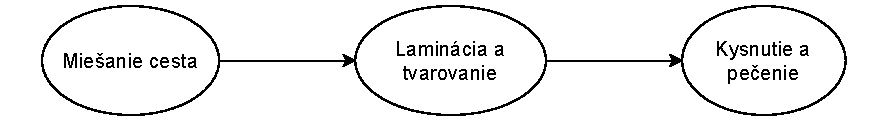
\includegraphics[width=0.9\linewidth]{croissant-process.pdf}
    \caption{Rozdelenie procesu výroby croissantov}
    \label{fig:croissant-process-diagram}
\end{figure}

Za každú časť zodpovedá práve jeden pekár ako je zobrazené v Petriho sieti na obrázku \ref{fig:petri-net}. V Petriho sieti nie je zobrazený presun pekára po skončení miešania na výpomoc pekárovi na kysnutie a pečenie. Tento proces je zobrazený na obrázku \ref{fig:mixer-baker-diagram}. Ďalej v Petriho sieti nie sú modelované poruchy strojov, ktoré sú implementované v simulatóri.

\begin{figure}[H]
    \centering
    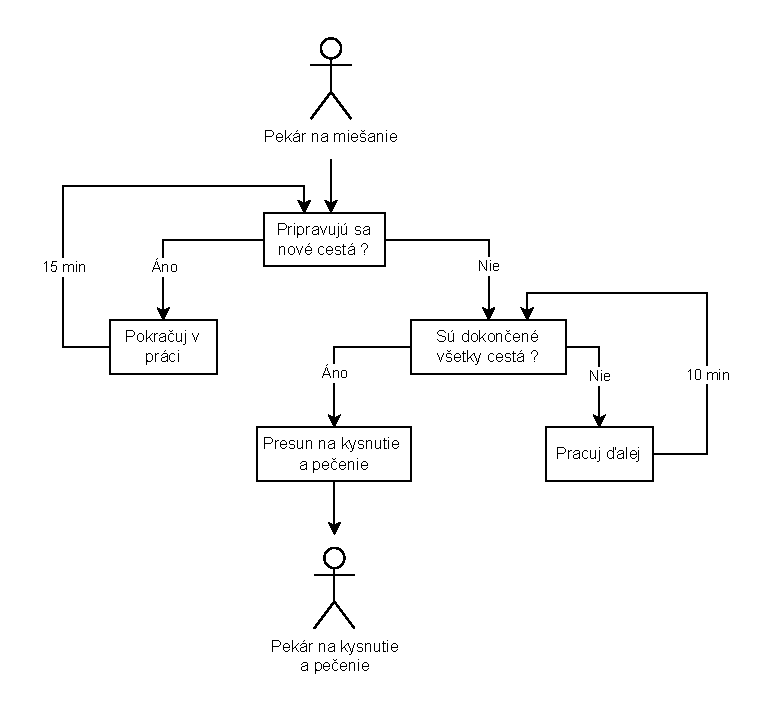
\includegraphics[width=0.8\linewidth]{mixer-baker-diagram.pdf}
    \caption{Diagram popisujúci prácu pekára zodpovedného za miešanie cesta}
    \label{fig:mixer-baker-diagram}
\end{figure}

\newpage
\section{Koncepcia simulátoru}
Architektúra simulátoru sa skladá z generátoru procesu cesta, pekárov, strojov a zariadení, prípadne generátorov pre poruchy strojov. Programom sa spúšťa simulácia jednej osemhodinovej zmeny v pekárni. Proces cesta simuluje jeho presun cez jednotlivé etapy spracovania cesta, po moment kedy sa z procesu cesta vytvoria procesy pre jednotlivé plechy. Pekári a stroje sú v programe implementované ako zariadenia, ktoré môže proces zabrať alebo čakať vo fronte na obslúženie. Zariadenia v pekárni sú implementované ako sklady s určitou kapacitou.

\subsection{Popis hlavných procesov}
Proces cesta sa špúsťa podľa intervalu daný normálnym rozložením so strednou hodnotou 15 minút a smerodatnou odchýlkou 2 minúty, po dobu 75 minút. Tieto parametre boli konfigurované podľa experimentu popísaného v \ref{exp:one_dough_experiment}. Po uplnutí tejto doby a dokončení všetkých úkonov spojených s miešaním sa pekár zodpovedný za miešanie presúva na výpomoc pekárovi na obsluhu a presun plechov.

Po tvarovaní cesta, proces cesta končí a v systéme pokračujú vytvorené procesy reprezentujúce plechy obsahujúce vytvarované croissanty, tento proces je popisaný algoritmom \ref{alg:create_trays_from_dough}.\newline

\begin{algorithm}[H]
\DontPrintSemicolon
\SetAlgoLined

\caption{Proces vytvárania plechov z cesta}
\label{alg:create_trays_from_dough}

pocet\_plnych\_plechov $\leftarrow$ pocet\_kusov / kapacita\_plechu\;
zvysne\_kusy $\leftarrow$ pocet\_kusov mod kapacita\_plechu\;

\If{zvysne\_kusy = 0}{
    \For{i $\leftarrow$ 0 \KwTo pocet\_plnych\_plechov - 1}{
        vytvor\_plech(kapacita\_plechu)\;
    }
    \Return\;
}
\Else{
    \If{zvysne\_kusy $>$ 0 \textbf{and} zvysne\_kusy $<$ 7 \textbf{and} pocet\_plnych\_plechov $>$ 0}{
        \For{i $\leftarrow$ 0 \KwTo pocet\_plnych\_plechov - 1}{
            naplnenie\_plechu $\leftarrow$ kapacita\_plechu\;
            \If{zvysne\_kusy $>$ 0}{
                naplnenie\_plechu $\leftarrow$ naplnenie\_plechu + 1\;
                zvysne\_kusy $\leftarrow$ zvysne\_kusy - 1\;
            }
            vytvor\_plech(naplnenie\_plechu)\;
        }
    }
    \Else{
        \For{i $\leftarrow$ 0 \KwTo pocet\_plnych\_plechov - 1}{
            vytvor\_plech(cas\_zaciatku, kapacita\_plechu)\;
        }
        vytvor\_plech(zvysne\_kusy)\;
    }
}

\end{algorithm}

\newpage
\section{Implementácia simulačného modelu}
Pri mapovaní koncepčného modelu na simulačný bol kladený dôraz na správnu simuláciu výrobného procesu a čo najpresnejšie simulovanie práce pekárov.

\subsection{Mapovanie koncepčného modelu}
Generovanie dávok cesta je implementované pomocou triedy \texttt{DoughGenerator}. Ak je simulačný čas menší ako hodnota parametru \texttt{DOBA\_GENEROVANIA\_NOVYCH\_CIEST} tak sa vytvorí nová inštancia triedy \texttt{Dough}, reprezentujúca proces cesta, ktorá sa zároveň aktivuje. Vygenerovanie ďalšej dávky cesta je naplánované za dobu danú normálnym rozložením so strednou hodnotu rovnej hodnote parametru \texttt{INTERVAL\_NOVEHO\_CESTA}.\newline

Pri konštrukcii procesu cesta sa vygeneruje množstvo kusov croissantov, ktoré z toho cesta vzniknú dané normálnym rozložením so strednou hodnotou rovnou hodnote parametru \texttt{POCET\_KUSOV\_Z\_JEDNEHO\_CESTA} a smerodatnou odchýlkou 2 kusy. Na konci procesu cesta sa vytvoria procesu reprezentujúce plechy naplnené vytvarovanými croissantami z tohto cesta.
Tento postup je popísaný v algoritme \ref{alg:create_trays_from_dough}.\newline

Generovanie porúch strojov je implementované v triedach \texttt{MixerFailure}, \texttt{LaminatorFailure}, \texttt{ShaperFailure}
a procesy opraváv v triedach \texttt{MixerRepair}, \texttt{LaminatorFailure}, \texttt{ShaperFailure}.

\subsection{Použité technológie}
Simulačný program bol implementovaný v programovacom jazyku \texttt{C++} podľa štandardu \texttt{c++20}. Na implementáciu modelu bola použitá simulačná knižnica \textsc{SIMLIB}. Táto knižnica implementuje prvky, využiteľné pre modelovanie systémov hromadnej obsluhy s paralelnými procesmi. Na preklad zdrojového kódu bol použitý prekladač \texttt{g++} spolu s nástrojom \texttt{Make}. 

\subsection{Spúšťanie simulácie}
 Simulačný program je potrebné pred spustením preložiť pomocou príkazu \texttt{make}. Po úspešnom preklade je spustenie simulácie nasledovné:
 
\begin{verbatim}
    ./simulation [parametre.csv]
\end{verbatim}

Bez zadania súboru so špecifikovanými parametrami simulácie sa použijú implicitné hodnoty modelu definované v zdrojovom kóde v súbore \texttt{paremeters.hpp}.\newline

V prípade použitia súboru sa implicitné hodnoty prepíšu hodnotami z \textsc{CSV} súboru, ktorého formát je nasledovný:

\begin{verbatim}
    NAZOV_PARAMETRU;HODNOTA_PARAMETRU
\end{verbatim}

Príkazom \texttt{make run} sa spustí simulácia s implicitnými hodnotami modelu. Príkazom \texttt{make sim} sa spustia simulácie všetkých experimentov v priečinku s názvom \texttt{sim}. Výsledky experimentov sú následne uložené do súborov s príponou \texttt{.out}.
 
\newpage
\section{Experimenty}
Pomocou experimentov bola vykonaná validácia modelu a prípadna úprava niektorých parametrov modelu. Cieľom experimentov bolo zistiť vyťaženosť jednotlivých strojov, zariadení a pekárov a zistiť slabé miesta vo výrobnej linke.
Nasledujúce experimenty boli zamerané na zistenie slabého miesta výroby, zachovanie úrovne produkcie pri možnom obmedzení niektorých zdrojov, možné zvýšenie produkcie pridaním zdrojov, prípadne následok poruchy strojov na celkovú produkciu počas jednej zmeny.
Vykonané experimenty by bez použitia modelu boli časovo a finančne náročné.

\subsection{Experiment 1}
\label{exp:one_dough_experiment}
V tomto experimente bolo za cieľ zistiť štatistiky o dobe výroby jedného cesta. Ná základe tohto experimentu bolo možné určiť hodnotu parameteru \texttt{DOBA\_GENEROVANIA\_NOVYCH\_CIEST}
a \texttt{INTERVAL\_NOVEHO\_CESTA}, tak aby sa linka nezahltila a stihli sa dorobiť všetky pripravené dávky do konca pracovnej zmeny. 

\begin{figure}[H]
\begin{verbatim}
    +----------------------------------------------------------+
    | HISTOGRAM Doba vyroby croisantov                         |
    +----------------------------------------------------------+
    | STATISTIC                                                |
    +----------------------------------------------------------+
    |  Min = 248.925                 Max = 291.771             |
    |  Number of records = 6                                   |
    |  Average value = 275.427                                 |
    +----------------------------------------------------------+
    |    from    |     to     |     n    |   rel    |   sum    |
    +------------+------------+----------+----------+----------+
    |    200.000 |    225.000 |        0 | 0.000000 | 0.000000 |
    |    225.000 |    250.000 |        1 | 0.166667 | 0.166667 |
    |    250.000 |    275.000 |        2 | 0.333333 | 0.500000 |
    |    275.000 |    300.000 |        3 | 0.500000 | 1.000000 |
    |    300.000 |    325.000 |        0 | 0.000000 | 1.000000 |
    |    325.000 |    350.000 |        0 | 0.000000 | 1.000000 |
    |    350.000 |    375.000 |        0 | 0.000000 | 1.000000 |
    |    375.000 |    400.000 |        0 | 0.000000 | 1.000000 |
    |    400.000 |    425.000 |        0 | 0.000000 | 1.000000 |
    |    425.000 |    450.000 |        0 | 0.000000 | 1.000000 |
    +------------+------------+----------+----------+----------+
\end{verbatim}
\caption{Štatistika doby výroby jedného cesta}
\label{fig:one_dough_experiment}
\end{figure}

Z vyššie uvedeného výpisu histogramu bolo zistené, že v prípade, keď sa počas simulácie v systéme nachádza len jedna dávka cesta, tak priemerná doba dokončenia plechu s croissantami je 275.427 minút. Z minimálnej a maximálnej hodnoty histogramu, môžeme ďalej uvažovať, že proces výroby trvá najmenej približne 250 minút a maximálne 300 minút. Počet záznamov v histograme 
odpovedá 6 naplneným plechom, ktoré vzniknú z jedného pripraveného cesta.

\newpage
\subsection{Experiment 2}
\label{exp:production_bottleneck_experiment}
Zmyslom tohto experimentu bolo zistiť slabé miesto výrobného procesu. Simulácia bola spúšťaná s nasledovnými implicitnými parametrami modelu.

\begin{verbatim}
    TRVANIE_SIMULACIE;480
    DOBA_GENEROVANIA_NOVYCH_CIEST;75
    INTERVAL_NOVEHO_CESTA;15
    POCET_KUSOV_Z_JEDNEHO_CESTA;300
    POCET_PEKAROV_NA_MIESANIE;1
    POCET_PEKAROV_NA_LAMINACIU_A_TVAROVANIE;1
    POCET_PEKAROV_NA_KYSNUTIE_A_PECENIE;1
    POCET_MIESACICH_STROJOV;1
    POCET_LAMINOVACICH_STROJOV;1
    POCET_TVAROVACICH_STROJOV;1
    KAPACITA_CHLADNICKY;8
    POCET_PLECHOV;30
    KAPACITA_PLECHU;50
    KAPACITA_KYSIARNE;40
    KAPACITA_PECE;5
\end{verbatim}

Na základe výpisov simulácie bol za najslabšie miesto, nazývané „bottleneck“, procesu výroby označený tvarovací stroj. Priemerná čakacia doba cesta na spracovanie tvarovacím strojom bola približne 70 minút, s minimálnou dobou čakania viac ako 50 minút.

\begin{figure}[H]
\begin{verbatim}
    +----------------------------------------------------------+
    | FACILITY tvarovaci_stroj_1                               |
    +----------------------------------------------------------+
    |  Status = not BUSY                                       |
    |  Time interval = 0 - 480                                 |
    |  Number of requests = 5                                  |
    |  Average utilization = 0.416641                          |
    +----------------------------------------------------------+
      Input queue 'tvarovaci_stroj_1.Q1'
    +----------------------------------------------------------+
    | QUEUE Q1                                                 |
    +----------------------------------------------------------+
    |  Time interval = 0 - 480                                 |
    |  Incoming  4                                             |
    |  Outcoming  4                                            |
    |  Current length = 0                                      |
    |  Maximal length = 3                                      |
    |  Average length = 0.586457                               |
    |  Minimal time = 56.546                                   |
    |  Maximal time = 75.947                                   |
    |  Average time = 70.3749                                  |
    +----------------------------------------------------------+
\end{verbatim}
\caption{Štatistika procesu výroby pri obmedzení zdrojov}
\label{fig:resources_limatation_experiment}
\end{figure}

\subsection{Experiment 3}
\label{exp:resources_limitation}
Cieľom tohto experimentu bolo zistiť možné obmedzenia jednotlivých zdrojov, pri zachovaní úrovne produkcie. Pri znížení nasledovných zdrojov sa výsledná produkcia nezmení, a teda je prípadne možné na týchto zdrojov ušetriť náklady.

\begin{verbatim}
    KAPACITA_CHLADNICKY;4
    POCET_PLECHOV;25
    KAPACITA_KYSIARNE;20
    KAPACITA_PECE;4
\end{verbatim}

Na nasledujúcom výpise, je možné vidieť, že výsledná produkcia výroby naozaj neklesla.

\begin{figure}[H]
\begin{verbatim}
    +----------------------------------------------------------+
    | STATISTICS vysledne pocty                                |
    +----------------------------------------------------------+
    |  Celkovy pocet ciest = 5                                 |
    |  Dokoncenych ciest = 5                                   |
    |                                                          |
    |  Celkovy pocet plechov = 30                              |
    |  Dokoncenych plechov = 30                                |
    |                                                          |
    |  Celkovy pocet kusov = 1498                              |
    |  Dokoncenych kusov = 1498                                |
    +----------------------------------------------------------+
\end{verbatim}
\caption{Štatistika procesu výroby pri obmedzení zdrojov}
\label{fig:resources_limatation_experiment}
\end{figure}

\subsection{Experiment 4}
\label{exp:mixer_failure_experiment}
Hlavným cieľom tohto experimentu bolo zdvojnásobiť produkciu croissantov v rámci jednej zmeny.

Ide o zväčšenie hodnoty parametru \texttt{DOBA\_GENEROVANIA\_NOVYCH\_CIEST} z pôvodnej hodnoty 75 na hodnotu 150, zdvojnásobenie strojov, pekárov a kapacity pece a pridanie ďalšich 20 plechov.

\begin{verbatim}
    DOBA_GENEROVANIA_NOVYCH_CIEST;150
     
    POCET_PEKAROV_NA_MIESANIE;2
    POCET_PEKAROV_NA_LAMINACIU_A_TVAROVANIE;2
    POCET_PEKAROV_NA_KYSNUTIE_A_PECENIE;2
    
    POCET_MIESACICH_STROJOV;2
    POCET_LAMINOVACICH_STROJOV;2
    POCET_TVAROVACICH_STROJOV;2
    
    POCET_PLECHOV;50
    KAPACITA_PECE;10
\end{verbatim}

\newpage
Na nasledujúcom výpise je možné pozorovať reálne zdvojnásobenie produkcie výroby.

\begin{figure}[H]
\begin{verbatim}
    +----------------------------------------------------------+
    | STATISTICS vysledne pocty                                |
    +----------------------------------------------------------+
    |  Celkovy pocet ciest = 10                                |
    |  Dokoncenych ciest = 10                                  |
    |                                                          |
    |  Celkovy pocet plechov = 60                              |
    |  Dokoncenych plechov = 60                                |
    |                                                          |
    |  Celkovy pocet kusov = 2987                              |
    |  Dokoncenych kusov = 2987                                |
    +----------------------------------------------------------+
\end{verbatim}
\caption{Štatistika procesu výroby pri obmedzení zdrojov}
\label{fig:resources_limatation_experiment}
\end{figure}

\subsection{Experiment 5}
\label{exp:laminator_failure_experiment}
V tomto experimente bol skúmaný vplyv poruchy miešacieho stroja na výslednú produkciu. Táto porucha je vygenerovaná náhodne medzi prvou a druhou tretinou doby počas, ktorej sa pripravujú nové cestá a jej oprava trvá približne 60 minút.

\begin{figure}[H]
\begin{verbatim}
    +----------------------------------------------------------+
    | STATISTICS vysledne pocty                                |
    +----------------------------------------------------------+
    |  Celkovy pocet ciest = 5                                 |
    |  Dokoncenych ciest = 4                                   |
    |                                                          |
    |  Celkovy pocet plechov = 24                              |
    |  Dokoncenych plechov = 24                                |
    |                                                          |
    |  Celkovy pocet kusov = 1196                              |
    |  Dokoncenych kusov = 1196                                |
    +----------------------------------------------------------+
\end{verbatim}
\caption{Štatistika procesu výroby pri poruche miešacieho stroja}
\label{fig:mixer_failure_experiment}
\end{figure}

Vo vyššie uvedenom výpise je dôležité si všimnúť rozdielny počet celkovo pripravených ciest a dokončených ciest, ktorý je spôsobený tým, že v prípade poruchy stroja, cesto ďalej nepokračuje vo výrobnom procese, ale je zahodené. Následne môžeme vidieť, že všetky ostatné cestá o počte 4, sa stihli dorobiť do konca zmeny.

\subsection{Experiment 6}
\label{exp:shaper_failure_experiment}
V nasledujúcom experimente bol skúmaný vplyv poruchy laminovacieho stroja medzi prvou a druhou tretinou celkovej doby výroby. Oprava stroja trvá približne 45 minút.

\begin{figure}[H]
\begin{verbatim}
    +----------------------------------------------------------+
    | STATISTICS vysledne pocty                                |
    +----------------------------------------------------------+
    |  Celkovy pocet ciest = 5                                 |
    |  Dokoncenych ciest = 5                                   |
    |                                                          |
    |  Celkovy pocet plechov = 30                              |
    |  Dokoncenych plechov = 30                                |
    |                                                          |
    |  Celkovy pocet kusov = 1495                              |
    |  Dokoncenych kusov = 1495                                |
    +----------------------------------------------------------+
\end{verbatim}
\caption{Štatistika procesu výroby pri poruche laminovacieho stroja}
\label{fig:mixer_failure_experiment}
\end{figure}

Z výpisu štatistík môžeme konštatovať, že porucha a jej následá oprava laminovacieho stroja nemala vplyv na výslednú produkciu.

\subsection{Experiment 7}
V poslednom experimente bolo skúmané ako ovplyvní porucha tvarovacieho stroja produkciu croissantov. Porucha je vygenerovaná náhodne medzi prvou a druhou tretinou celkovej doby výroby. Oprava stroja trvá približne 25 minút.

\begin{figure}[H]
\begin{verbatim}
    +----------------------------------------------------------+
    | STATISTICS vysledne pocty                                |
    +----------------------------------------------------------+
    |  Celkovy pocet ciest = 5                                 |
    |  Dokoncenych ciest = 4                                   |
    |                                                          |
    |  Celkovy pocet plechov = 24                              |
    |  Dokoncenych plechov = 22                                |
    |                                                          |
    |  Celkovy pocet kusov = 1196                              |
    |  Dokoncenych kusov = 1096                                |
    +----------------------------------------------------------+
\end{verbatim}
\caption{Štatistika procesu výroby pri poruche tvarovacieho stroja}
\label{fig:mixer_failure_experiment}
\end{figure}

Z výpisu štatistík tohto experimentu je vidieť najväčší vplyv na výslednú produkciu, spomedzi porúch jednotlivých strojov. Z celkového počtu piatich ciest len štyri pokračujú v procese výroby, z ktorých je dokončených len 22 plechov z celkových 24 plechov. S počtu dokončených kusov môžeme konštatovať pokles produkcie o približne 400 kusov oproti referenčnej produkcii. 

\newpage
\section{Záver}
Táto práca popísala tvorbu modelu malej pekárne na výrobu croissantov. Z výsledkov experimentu bolo zistené, že pre dosiahnutie produkcie 1500 kusov za jednu osemhodinnovú zmenu je potrebné pripravovať nové cestá v intervale 15 minút po dobu 75 minút. Za najslabšie miesto celkovej výroby bol zistený tvarovací stroj s priemernou dlžkou čakacej doby 70 minút. Ďalej bolo zistené, že je možné obmedziť naledovné zdroje pri zachovaní úrovne produkcie, zmenšiť kapacitu chladničky a kysiarne o polovicu a kapacitu pece o 1 plech, pričom stačí 25 plechov namiesto pôvodných 30. Rovnako boli zistené potrebné navýšenia zdrojov pre zdvojnásobenie produkcie a vplyv porúch strojov na výrobu. Validita modelu bola overená vykonaním experimentov a konzultáciou s človekom z oboru. V rámci tejto práce vznikol model, ktorý by mohol pomôcť k zlepšeniu výrobného procesu croissantov.

\newpage
\printbibliography[title={Použitá literatúra}]

\newpage
\appendix

\section{Petriho sieť}
\begin{figure}[H]
    \centering
    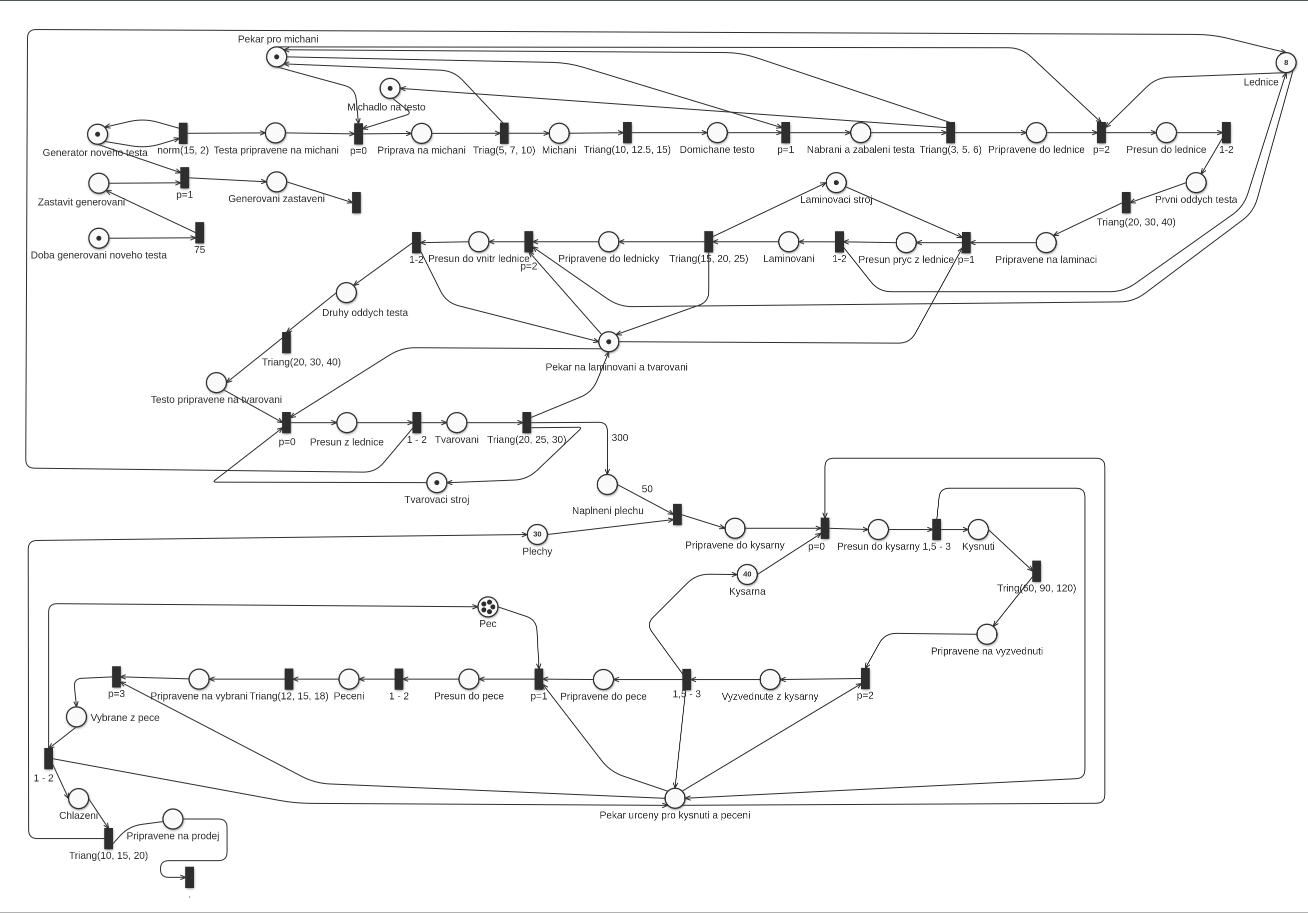
\includegraphics[width=0.9\textwidth]{petri-net.png}
    \label{fig:petri-net}
\end{figure}

\end{document}